% Copyright 2006 by Till Tantau
%
% This file may be distributed and/or modified
%
% 1. under the LaTeX Project Public License and/or
% 2. under the GNU Free Documentation License.
%
% See the file doc/generic/pgf/licenses/LICENSE for more details.


\section{Tutorial: Euclid's Amber Version of the \emph{Elements}}

In this third tutorial we have a look at how \tikzname\ can be used to
draw geometric constructions.

Euclid is currently quite busy writing his new book series, whose
working title is ``Elements'' (Euclid is not quite sure whether this
title will convey the message of the series to future generations
correctly, but he intends to change the title before it goes to the
publisher). Up to know, he wrote down his text and graphics on
papyrus, but his publisher suddenly insists that he must submit in
electronic form. Euclid tries to argue with the publisher that 
electronics will only be discovered thousands of years later, but the
publisher informs him that the use of amber is no longer cutting edge
technology and Euclid will just have to keep up with modern tools.

Slightly disgruntled, Euclid starts converting his papyrus
entitled ``Book I, Proposition I'' to an amber version.  

\subsection{Book I, Proposition I}

The drawing on his papyrus looks like this:\footnote{The text is taken
from the wonderful interactive version of Euclid's Elements by David
E. Joyce, to be found on his website at Clark University.}

\bigskip
\noindent
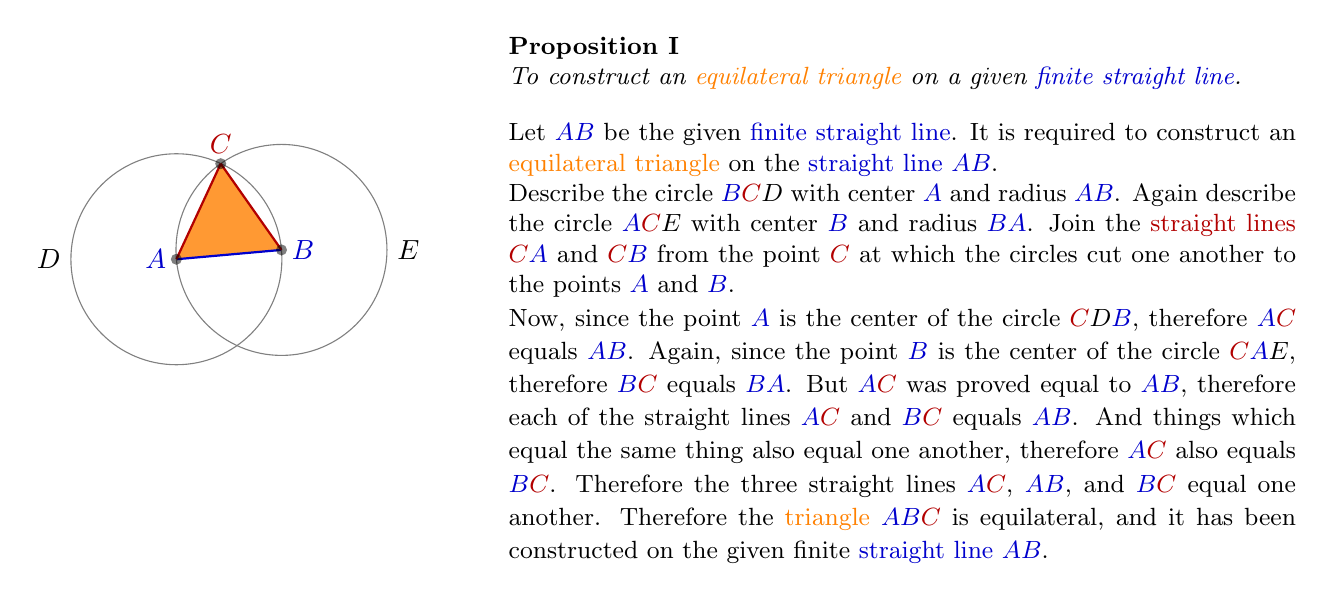
\begin{tikzpicture}[thick,help lines/.style={thin,draw=black!50}]
  \def\A{\textcolor{input}{$A$}}
  \def\B{\textcolor{input}{$B$}}
  \def\C{\textcolor{output}{$C$}}
  \def\D{$D$}
  \def\E{$E$}
  
  \colorlet{input}{blue!80!black}
  \colorlet{output}{red!70!black}
  \colorlet{triangle}{orange}
  
  \coordinate [label=left:\A]
    (A) at ($ (0,0) + .1*(rand,rand) $);
  \coordinate [label=right:\B]
    (B) at ($ (1.25,0.25) + .1*(rand,rand) $);

  \draw [input] (A) -- (B);
  
  \node [help lines,draw,label=left:\D] (D) at (A) [circle through=(B)] {};
  \node [help lines,draw,label=right:\E] (E) at (B) [circle through=(A)] {};
  
  \coordinate [label=above:\C]
    (C) at (intersection 2 of D and E);

  \draw [output] (A) -- (C);
  \draw [output] (B) -- (C);

  \foreach \point in {A,B,C}
    \fill [black,opacity=.5] (\point) circle (2pt);

  \begin{pgfonlayer}{background}
    \fill[triangle!80] (A) -- (C) -- (B) -- cycle;
  \end{pgfonlayer}
  
  \node [below right,text width=10cm,text justified] at (4,3)
  {
    \small
    \textbf{Proposition I}\par
    \emph{To construct an \textcolor{triangle}{equilateral triangle}
      on a given \textcolor{input}{finite straight line}.}
    \par
    \vskip1em
    Let \A\B\ be the given \textcolor{input}{finite straight line}. It
    is required to construct an \textcolor{triangle}{equilateral
      triangle} on the \textcolor{input}{straight line}~\A\B. 

    Describe the circle \B\C\D\ with center~\A\ and radius \A\B. Again
    describe the circle \A\C\E\ with center~\B\ and radius \B\A. Join the
    \textcolor{output}{straight lines} \C\A\ and \C\B\ from the
    point~\C\ at which the circles cut one another to the points~\A\ and~\B.

    Now, since the point~\A\ is the center of the circle \C\D\B,
    therefore \A\C\ equals \A\B. Again, since the point \B\ is the
    center of the circle \C\A\E, therefore \B\C\ equals \B\A. But
    \A\C\ was proved equal to \A\B, therefore each of the straight
    lines \A\C\ and \B\C\ equals \A\B. And 
    things which equal the same thing also equal one another,
    therefore \A\C\ also equals \B\C. Therefore the three straight
    lines \A\C, \A\B, and \B\C\ equal one another. 
    Therefore the \textcolor{triangle}{triangle} \A\B\C\ is
    equilateral, and it has been  constructed on the given finite
    \textcolor{input}{straight line}~\A\B.  
  };
\end{tikzpicture}
\bigskip

Let us have a look at how Euclid can turn this into \tikzname\ code.

\subsubsection{Setting up the Environment}

As in the previous tutorials, Euclid needs to load \tikzname, together
with some libraries. These libraries are |calc|, |through|, and
|backgrounds|. Depending on which format he uses, Euclid would use one
of the following in the preamble: 

\begin{codeexample}[code only]
% For LaTeX:
\usepackage{tikz}
\usetikzlibrary{calc,through,backgrounds}
\end{codeexample}

\begin{codeexample}[code only]
% For plain TeX:
\input tikz.tex
\usetikzlibrary{calc,through,backgrounds}
\end{codeexample}

\begin{codeexample}[code only]
% For ConTeXt:
\usemodule[tikz]
\usetikzlibrary[calc,through,backgrounds]
\end{codeexample}


\subsubsection{The Line \emph{AB}}

The first part of the picture that Euclid wishes to draw is the line
$AB$. That is easy enough, something like |\draw (0,0) -- (2,1);|
might do. However, Euclid does not wish to reference the two points
$A$ and $B$ as $(0,0)$ and $(2,1)$ subsequently. Rather, he wishes to
just write |A| and |B|. Indeed, the whole point of his book is that
the points $A$ and $B$ can be arbitrary and all other points (like
$C$) are constructed in terms of their positions. It would not do
if Euclid were to write down the coordinates of $C$ explicitly.

So, Euclid starts with defining two coordinates using the
|\coordinate| command:
\begin{codeexample}[]
\begin{tikzpicture}
  \coordinate (A) at (0,0);
  \coordinate (B) at (1.25,0.25);

  \draw[blue] (A) -- (B);
\end{tikzpicture}
\end{codeexample}

That was easy enough. What is missing at this point are the labels for
the coordinates. Euclid does not want them \emph{on} the points, but
next to them. He decides to use the |label| option:
\begin{codeexample}[]
\begin{tikzpicture}
  \coordinate [label=left:\textcolor{blue}{$A$}]  (A) at (0,0);
  \coordinate [label=right:\textcolor{blue}{$B$}] (B) at (1.25,0.25);

  \draw[blue] (A) -- (B);
\end{tikzpicture}
\end{codeexample}

At this point, Euclid decides that it would be even nicer if the
points $A$ and $B$ were in some sense ``random.'' Then, neither Euclid
nor the reader can make the mistake of taking ``anything for granted''
concerning these position of these points. Euclid is pleased to learn
that there is a |rand| function in \tikzname\ that does exactly what
he needs: It produces a number between $-1$ and $1$. Since \tikzname\
can do a bit of math, Euclid can change the coordinates of the points
as follows:
\begin{codeexample}[code only]
\coordinate [...] (A) at (0+0.1*rand,0+0.1*rand);
\coordinate [...] (B) at (1.25+0.1*rand,0.25+0.1*rand);
\end{codeexample}

This works fine. However, Euclid is not quite satisfied since he would
prefer that the ``main coordinates'' $(0,0)$ and $(1.25,0.25)$ are
``kept separate'' from the perturbation
$0.1(\mathit{rand},\mathit{rand})$. This means, he would like to
specify that coordinate $A$ as ``The point that is at $(0,0)$ plus one
tenth of the vector  $(\mathit{rand},\mathit{rand})$.''

It turns out that the |calc| library allows him to do exactly this
kind of computation. When this library is loaded, you can use special
coordinates that start with |($| and end with |$)| rather than just
|(| and~|)|. Inside these special coordinates you can give a linear
combination of coordinates. (Note that the dollar signs are only
intended to signal that a ``computation'' is going on; no mathematical
typesetting is done.)

The new code for the coordinates is the following:

\begin{codeexample}[code only]
\coordinate [...] (A) at ($ (0,0) + .1*(rand,rand) $);
\coordinate [...] (B) at ($ (1.25,0.25) + .1*(rand,rand) $);
\end{codeexample}

Note that if a coordinate in such a computation has a factor (like
|.1|) you must place a |*| directly before the opening parenthesis of
the coordinate. You can nest such computations.



\subsubsection{The Circle Around \emph{A}}

The first tricky construction is the circle around~$A$. We will see
later how to do this in a very simple manner, but first let us do it
the ``hard'' way.

The idea is the following: We draw a circle around the point $A$ whose
radius is given by the length of the line $AB$. The difficulty lies in
computing the length of this line.

Two ideas ``nearly'' solve this problem: First, we can write
|($ (A) - (B) $)| for the vector that is the difference between $A$
and~$B$. All we need is the length of this vector. Second, given two
numbers $x$ and $y$, one can write |veclen(|$x$|,|$y$|)| inside a
mathematical expression. This gives the value $\sqrt{x^2+y^2}$, which
is exactly the desired length.

The only remaining problem is to access the $x$- and $y$-coordinate of
the vector~$AB$. For this, we need a new concept: the \emph{let
  operation}. A let operation can be given anywhere on a path where a
normal path operation like a line-to or a move-to is expected. The
effect of a let operation is to evaluate some coordinates and to
assign the results to special macros. These macros make it easy to
access the $x$- and $y$-coordinates of the coordinates.

Euclid would write the following:
\begin{codeexample}[]
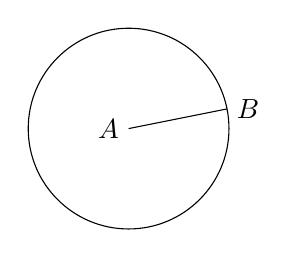
\begin{tikzpicture}
  \coordinate [label=left:$A$]  (A) at (0,0);
  \coordinate [label=right:$B$] (B) at (1.25,0.25);
  \draw (A) -- (B);

  \draw (A) let
              \p1 = ($ (B) - (A) $)
            in
              circle ({veclen(\x1,\y1)});
\end{tikzpicture}
\end{codeexample}

Each assignment in a let operation starts with |\p|, usually followed
by a \meta{digit}. Then comes an equal sign and a coordinate. The
coordinate is evaluated and the result is stored internally. From
then on you can use the following expressions: 
\begin{enumerate}
\item |\x|\meta{digit} yields the $x$-coordinate of the resulting point.
\item |\y|\meta{digit} yields the $y$-coordinate of the resulting
  point.
\item |\p|\meta{digit} yields the same as |\x|\meta{digit}|,\y|\meta{digit}.
\end{enumerate}
You can have multiple assignments in a let operation, just separate
them with commas. In later assignments you can already use the results
of earlier assignments.

Note that |\p1| is not a coordinate in the usual sense. Rather, it
just expands to a string like |10pt,20pt|. So, you cannot write, for
instance, |(\p1.center)| since this would just expand to
|(10pt,20pt.center)|, which makes no sense.

Next, we want to draw both circles at the same time. Each time the
radius is |veclen(\x1,\y1)|. It seems natural to compute this radius
only once. For this, we can also use a let operation: Instead of
writing |\p1 = ...|, we write |\n2 = ...|. Here, ``n'' stands for
``number'' (while ``p'' stands for ``point''). The assignment of a
number should be followed by a number in curly braces.
\begin{codeexample}[]
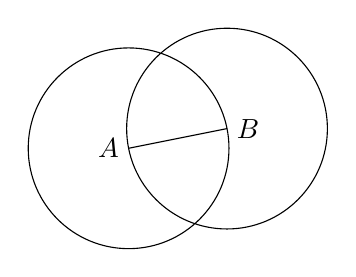
\begin{tikzpicture}
  \coordinate [label=left:$A$]  (A) at (0,0);
  \coordinate [label=right:$B$] (B) at (1.25,0.25);
  \draw (A) -- (B);

  \draw let \p1 = ($ (B) - (A) $),
            \n2 = {veclen(\x1,\y1)}
        in
          (A) circle (\n2)
          (B) circle (\n2);
\end{tikzpicture}
\end{codeexample}
In the above example, you may wonder, what |\n1| would yield? The
answer is that it would be undefined -- the |\p|, |\x|, and |\y|
macros refer to the same logical point, while the |\n| macro has ``its
own namespace.'' We could even have replaced |\n2| in the example by
|\n1| and it would still work. Indeed, the digits following these
macros are just normal \TeX\ parameters. We could also use a longer
name, but then we have to use curly braces:
\begin{codeexample}[]
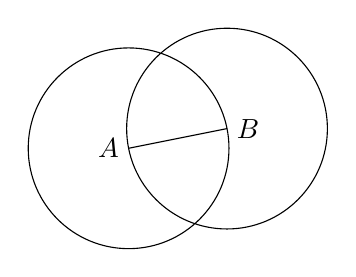
\begin{tikzpicture}
  \coordinate [label=left:$A$]  (A) at (0,0);
  \coordinate [label=right:$B$] (B) at (1.25,0.25);
  \draw (A) -- (B);

  \draw let \p1        = ($ (B) - (A) $),
            \n{radius} = {veclen(\x1,\y1)}
        in
          (A) circle (\n{radius})
          (B) circle (\n{radius});
\end{tikzpicture}
\end{codeexample}

At the beginning of this section it was promised that there is an
easier way to create the desired circle. The trick is to use the
|through| library. As the name suggests, it contains code for creating
shapes that go through a given point.

The option that we are looking for is |circle through|. This option is
given to a \emph{node} and has the following effects: First, it causes
the node's inner and outer separations to be set to zero. Then it sets
the shape of the node to |circle|. Finally, it sets the radius of the
node such that it goes through the parameter given to
|circle through|. This radius is computed in essentially the same way
as above.

\begin{codeexample}[]
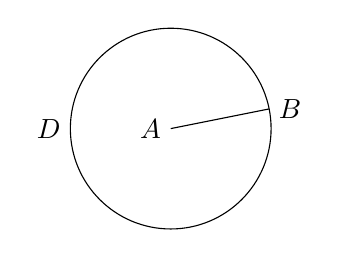
\begin{tikzpicture}
  \coordinate [label=left:$A$]  (A) at (0,0);
  \coordinate [label=right:$B$] (B) at (1.25,0.25);
  \draw (A) -- (B);

  \node [draw,circle through=(B),label=left:$D$] at (A) {};
\end{tikzpicture}
\end{codeexample}


\subsubsection{The Intersection of the Circles}

Euclid can now draw the line and the circles. The final problem is to
compute the intersection of the two circles. This computation is a bit
involved if you want to do it ``by hand.'' Fortunately, the so-called
intersection coordinate system allows us to specify points as the
intersection of two objects (in order for the following code to work,
the |calc| library must be loaded; it defines the necessary code for
computing the intersection of circles):
\begin{codeexample}[]
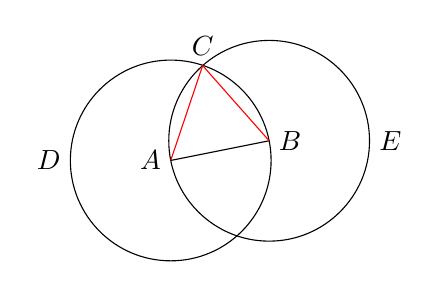
\begin{tikzpicture}
  \coordinate [label=left:$A$]  (A) at (0,0);
  \coordinate [label=right:$B$] (B) at (1.25,0.25);
  \draw (A) -- (B);

  \node (D) [draw,circle through=(B),label=left:$D$]  at (A) {};
  \node (E) [draw,circle through=(A),label=right:$E$] at (B) {};

  \coordinate [label=above:$C$] (C) at (intersection 2 of D and E);

  \draw [red] (A) -- (C);
  \draw [red] (B) -- (C);
\end{tikzpicture}
\end{codeexample}

We could also have written |intersection 1 of| or just
|intersection of| to get access to the other intersection of the
circles.

Although Euclid does not need it for the current picture, it is just a
small step to computing the bisection of the line $AB$:

\begin{codeexample}[]
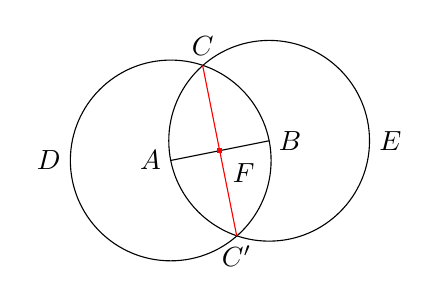
\begin{tikzpicture}
  \coordinate [label=left:$A$]  (A) at (0,0);
  \coordinate [label=right:$B$] (B) at (1.25,0.25);
  \draw (A) -- (B);

  \node (D) [draw,circle through=(B),label=left:$D$]  at (A) {};
  \node (E) [draw,circle through=(A),label=right:$E$] at (B) {};

  \coordinate [label=above:$C$]  (C)  at (intersection 2 of D and E);
  \coordinate [label=below:$C'$] (C') at (intersection 1 of D and E);

  \draw [red] (C) -- (C');
  \node [fill=red,inner sep=1pt,label=-45:$F$] (F) at (intersection of C--C' and A--B) {};
\end{tikzpicture}
\end{codeexample}



\subsubsection{The Complete Code}

Back to Euclid's code. He introduces a few macros to make life
simpler, like a |\A| macro for typesetting a blue $A$. He also uses the
|background| layer for drawing the triangle behind everything at the
end. 

\begin{codeexample}[]
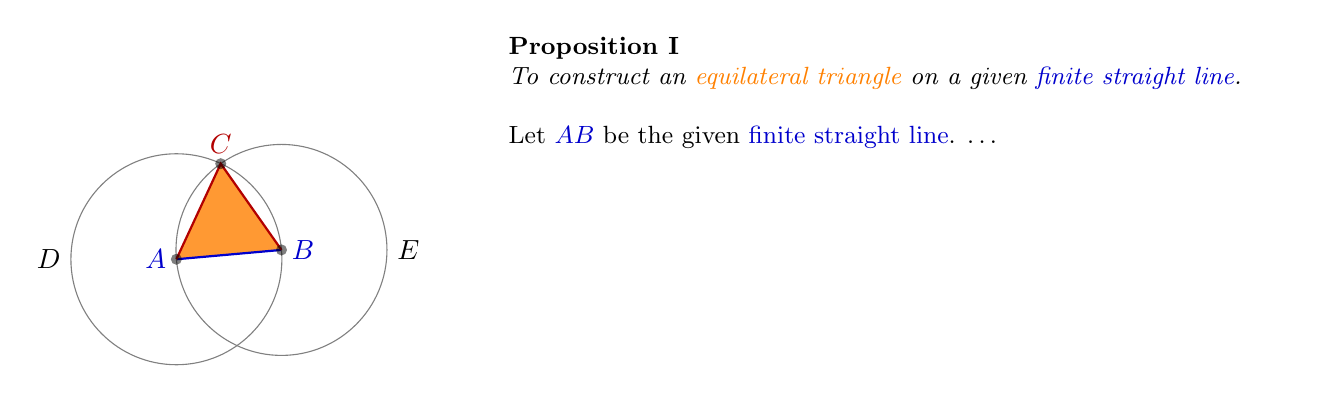
\begin{tikzpicture}[thick,help lines/.style={thin,draw=black!50}]
  \def\A{\textcolor{input}{$A$}}     \def\B{\textcolor{input}{$B$}}
  \def\C{\textcolor{output}{$C$}}    \def\D{$D$}
  \def\E{$E$}
  
  \colorlet{input}{blue!80!black}    \colorlet{output}{red!70!black}
  \colorlet{triangle}{orange}
  
  \coordinate [label=left:\A]  (A) at ($ (0,0) + .1*(rand,rand) $);
  \coordinate [label=right:\B] (B) at ($ (1.25,0.25) + .1*(rand,rand) $);

  \draw [input] (A) -- (B);
  
  \node [help lines,draw,label=left:\D]   (D) at (A) [circle through=(B)] {};
  \node [help lines,draw,label=right:\E]  (E) at (B) [circle through=(A)] {};
  
  \coordinate [label=above:\C] (C) at (intersection 2 of D and E);

  \draw [output] (A) -- (C) -- (B);

  \foreach \point in {A,B,C}
    \fill [black,opacity=.5] (\point) circle (2pt);

  \begin{pgfonlayer}{background}
    \fill[triangle!80] (A) -- (C) -- (B) -- cycle;
  \end{pgfonlayer}
  
  \node [below right, text width=10cm,text justified] at (4,3) {
    \small\textbf{Proposition I}\par
    \emph{To construct an \textcolor{triangle}{equilateral triangle}
      on a given \textcolor{input}{finite straight line}.}
    \par\vskip1em
    Let \A\B\ be the given \textcolor{input}{finite straight line}.  \dots
  };
\end{tikzpicture}
\end{codeexample}


\subsection{Book I, Proposition II}

The second proposition in the Elements is the following:

\bigskip\noindent
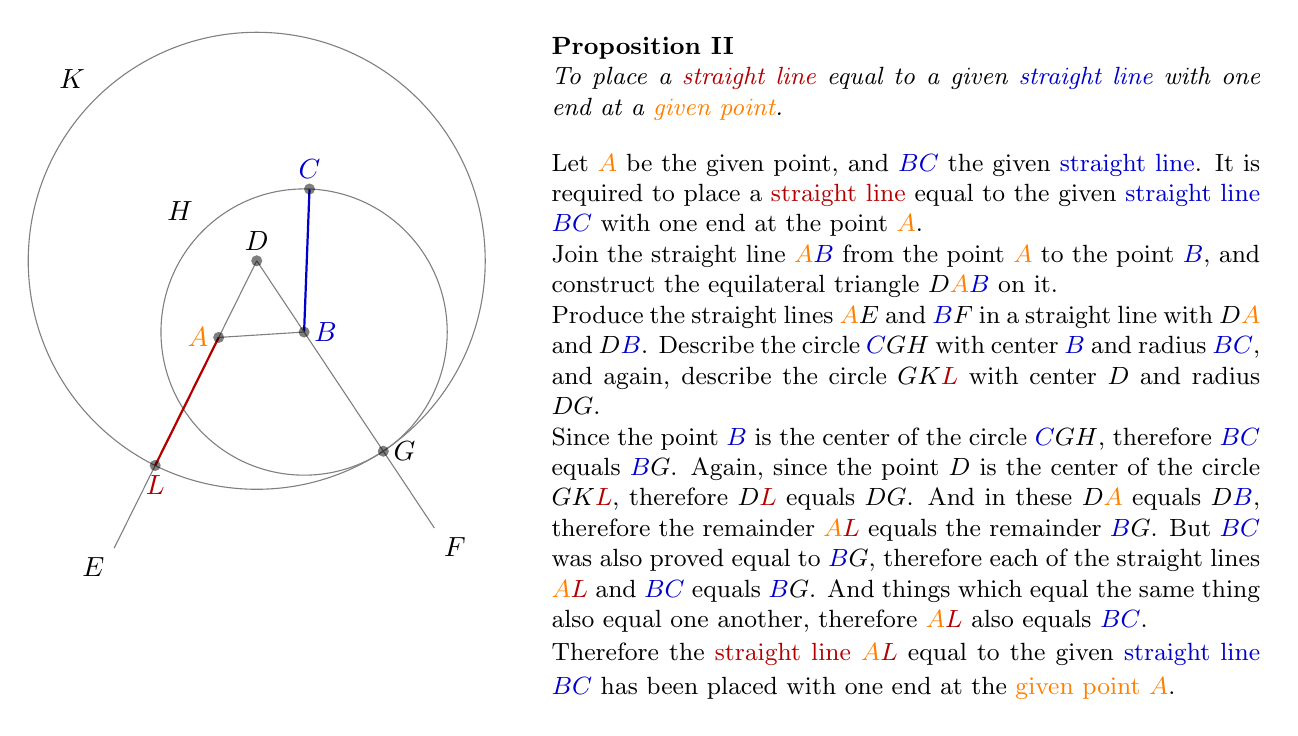
\begin{tikzpicture}[thick,help lines/.style={thin,draw=black!50}]
  \def\A{\textcolor{orange}{$A$}}   \def\B{\textcolor{input}{$B$}}
  \def\C{\textcolor{input}{$C$}}    \def\D{$D$}
  \def\E{$E$}                       \def\F{$F$}
  \def\G{$G$}                       \def\H{$H$}
  \def\K{$K$}                       \def\L{\textcolor{output}{$L$}}
  
  \colorlet{input}{blue!80!black}    \colorlet{output}{red!70!black}
  
  \coordinate [label=left:\A]  (A) at ($ (0,0) + .1*(rand,rand) $);
  \coordinate [label=right:\B] (B) at ($ (1,0.2) + .1*(rand,rand) $);
  \coordinate [label=above:\C] (C) at ($ (1,2) + .1*(rand,rand) $);

  \draw [input] (B) -- (C);
  \draw [help lines] (A) -- (B);

  \coordinate [label=above:\D] (D) at ($ (A)!.5!(B) ! {sin(60)*2} ! 90:(B) $);

  \draw [help lines] (D) -- ($ (D)!3.75!(A) $) coordinate [label=-135:\E] (E);
  \draw [help lines] (D) -- ($ (D)!3.75!(B) $) coordinate [label=-45:\F] (F);

  \node (H) at (B) [help lines,circle through=(C),draw,label=135:\H] {};

  \coordinate [label=right:\G] (G) at (intersection of B--F and H);

  \node (K) at (D) [help lines,circle through=(G),draw,label=135:\K] {};

  \coordinate [label=below:\L] (L) at (intersection of A--E and K);

  \draw [output] (A) -- (L);

  \foreach \point in {A,B,C,D,G,L}
    \fill [black,opacity=.5] (\point) circle (2pt);
  
  \node [below right, text width=9cm,text justified] at (4,4) {
    \small\textbf{Proposition II}\par
    \emph{To place a \textcolor{output}{straight line} equal to a
      given \textcolor{input}{straight line} with 
      one end at a \textcolor{orange}{given point}.} 
    \par\vskip1em
    Let \A\ be the given point, and \B\C\ the given
    \textcolor{input}{straight line}. 
    It is required to place a \textcolor{output}{straight line} equal
    to the given \textcolor{input}{straight line} \B\C\ with one end
    at the point~\A.  

    Join the straight line \A\B\ from the point \A\ to the point \B, and
    construct the equilateral triangle \D\A\B\ on it.
    
    Produce the straight lines \A\E\ and \B\F\ in a straight line with
    \D\A\ and \D\B. Describe the circle \C\G\H\ with center \B\ and
    radius \B\C, and  again, describe the circle \G\K\L\ with center
    \D\ and radius \D\G. 	

    Since the point \B\ is the center of the circle \C\G\H, therefore
    \B\C\ equals \B\G. Again, since the point \D\ is the center of the
    circle \G\K\L, therefore \D\L\ equals \D\G. And in these \D\A\
    equals \D\B, therefore the remainder \A\L\ equals the remainder
    \B\G. But \B\C\ was also proved  equal to \B\G, therefore each of
    the straight lines \A\L\ and \B\C\ equals \B\G. And things which
    equal the same thing also equal one another, therefore \A\L\ also
    equals \B\C. 
    
    Therefore the \textcolor{output}{straight line} \A\L\ equal to the
    given \textcolor{input}{straight line} \B\C\  has been placed with
    one end at the \textcolor{orange}{given point}~\A.  
  };
\end{tikzpicture}




\subsubsection{Using Partway Calculations for the Construction of \emph{D}}

Euclid's construction starts with ``referencing'' Proposition~I for
the construction of the point~$D$. Now, while we could simply repeat the
construction, it seems a bit bothersome that one has to draw all these
circles and do all these complicated constructions.

For this reason, \tikzname\ supports some simplifications. First,
there is a simple syntax for computing a point that is ``partway'' on
a line from $p$ to~$q$: You place these two points in a coordinate
calculation -- remember, they start with |($| and end with |$)| -- and
then combine them using |!|\meta{part}|!|. A \meta{part} of |0| refers
to the \emph{first} coordinate, a \meta{part} of |1| refers to the
second coordinate, and a value in between refers to a point on the
line from $p$ to~$q$. Thus, the syntax is similar to the |xcolor|
syntax for mixing colors.

Here is the computation of the point in the middle of the line $AB$:
\begin{codeexample}[]
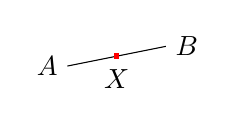
\begin{tikzpicture}
  \coordinate [label=left:$A$]  (A) at (0,0);
  \coordinate [label=right:$B$] (B) at (1.25,0.25);
  \draw (A) -- (B);
  \node [fill=red,inner sep=1pt,label=below:$X$] (X) at ($ (A)!.5!(B) $) {};
\end{tikzpicture}
\end{codeexample}

The computation of the point $D$ in Euclid's second proposition is a
bit more complicated. It can be expressed as follows: Consider the
line from $X$ to $B$. Suppose we 
rotate this line around $X$ for 90$^\circ$ and then stretch it by a
factor of $\sin(60^\circ)/2$. This yields the desired point~$D$. We
can do the stretching using the partway modifier above, for the
rotation we need a new modifier: the rotation modifier. The idea is
that the second coordinate in a partway computation can be prefixed by
an angle. Then the partway point is computed normally (as if no angle
were given), but the resulting point is rotated by this angle around
the first point.  

\begin{codeexample}[]
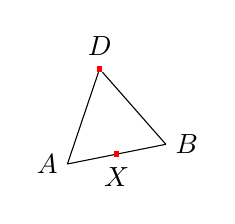
\begin{tikzpicture}
  \coordinate [label=left:$A$]  (A) at (0,0);
  \coordinate [label=right:$B$] (B) at (1.25,0.25);
  \draw (A) -- (B);
  \node [fill=red,inner sep=1pt,label=below:$X$] (X) at ($ (A)!.5!(B) $) {};
  \node [fill=red,inner sep=1pt,label=above:$D$] (D) at
    ($ (X) ! {sin(60)*2} ! 90:(B) $) {};
  \draw (A) -- (D) -- (B);
\end{tikzpicture}
\end{codeexample}

Finally, it is not necessary to explicitly name the point $X$. Rather,
again like in the |xcolor| package, it is possible to chain partway
modifiers:

\begin{codeexample}[]
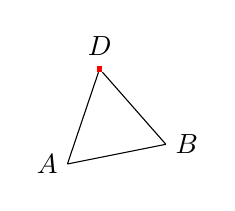
\begin{tikzpicture}
  \coordinate [label=left:$A$]  (A) at (0,0);
  \coordinate [label=right:$B$] (B) at (1.25,0.25);
  \draw (A) -- (B);
  \node [fill=red,inner sep=1pt,label=above:$D$] (D) at
    ($ (A) ! .5 ! (B) ! {sin(60)*2} ! 90:(B) $) {};
  \draw (A) -- (D) -- (B);
\end{tikzpicture}
\end{codeexample}


\subsubsection{Intersecting a Line and a Circle}

The next step in the construction is to draw a circle around $B$
through $C$, which is easy enough to do using the |circle through|
option. Extending the lines $DA$ and $DB$ can be done using partway
calculations, but this time with a part value outside the range
$[0,1]$: 

\begin{codeexample}[]
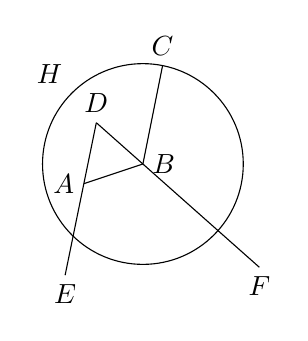
\begin{tikzpicture}
  \coordinate [label=left:$A$]  (A) at (0,0);
  \coordinate [label=right:$B$] (B) at (0.75,0.25);
  \coordinate [label=above:$C$] (C) at (1,1.5);
  \draw (A) -- (B) -- (C);
  \coordinate [label=above:$D$] (D) at
    ($ (A) ! .5 ! (B) ! {sin(60)*2} ! 90:(B) $) {};
  \node (H) [label=135:$H$,draw,circle through=(C)] at (B) {};
  \draw (D) -- ($ (D) ! 3.5 ! (B) $) coordinate [label=below:$F$] (F);
  \draw (D) -- ($ (D) ! 2.5 ! (A) $) coordinate [label=below:$E$] (E);
\end{tikzpicture}
\end{codeexample}

We now face the problem of finding the point $G$, which is the
intersection of the line $BF$ and the circle $H$. One way is to use
yet another variant of the partway computation: Normally, a partway
computation has the form \meta{p}|!|\meta{factor}|!|\meta{q},
resulting in the point $(1-\meta{factor})\meta{p} +
\meta{factor}\meta{q}$. Alternatively, instead of \meta{factor} you
can also use a \meta{dimension} between the points. In this case, you
get the point that is \meta{dimension} removed from \meta{p} on the
straight line to \meta{q}.

We know that the point $G$ is on the way from $B$ to $F$. The distance
is given by the radius of the circle~$H$. Here is the code form
computing $H$:
\begin{codeexample}[pre={
\begin{tikzpicture}
  \coordinate [label=left:$A$]  (A) at (0,0);
  \coordinate [label=right:$B$] (B) at (0.75,0.25);
  \coordinate [label=above:$C$] (C) at (1,1.5);
  \draw (A) -- (B) -- (C);
  \coordinate [label=above:$D$] (D) at
    ($ (A) ! .5 ! (B) ! {sin(60)*2} ! 90:(B) $) {};
  \node (H) [label=135:$H$,draw,circle through=(C)] at (B) {};
  \draw (D) -- ($ (D) ! 3.5 ! (B) $) coordinate [label=below:$F$] (F);
  \draw (D) -- ($ (D) ! 2.5 ! (A) $) coordinate [label=below:$E$] (E);
},post={\end{tikzpicture}}]
  \path let \p1 = ($ (B) - (C) $) in
    coordinate [label=left:$G$] (G) at ($ (B) ! veclen(\x1,\y1) ! (F) $);
  \fill[red,opacity=.5] (G) circle (2pt);
\end{codeexample}

However, there is a simpler way: As for circles, we can also intersect
a line and a circle using the |intersection| coordinate system:

\begin{codeexample}[pre={
\begin{tikzpicture}
  \coordinate [label=left:$A$]  (A) at (0,0);
  \coordinate [label=right:$B$] (B) at (0.75,0.25);
  \coordinate [label=above:$C$] (C) at (1,1.5);
  \draw (A) -- (B) -- (C);
  \coordinate [label=above:$D$] (D) at
    ($ (A) ! .5 ! (B) ! {sin(60)*2} ! 90:(B) $) {};
  \node (H) [label=135:$H$,draw,circle through=(C)] at (B) {};
  \draw (D) -- ($ (D) ! 3.5 ! (B) $) coordinate [label=below:$F$] (F);
  \draw (D) -- ($ (D) ! 2.5 ! (A) $) coordinate [label=below:$E$] (E);
},post={\end{tikzpicture}}]
  \coordinate [label=left:$G$] (G) at (intersection of B--F and H);
  \fill[red,opacity=.5] (G) circle (2pt);
\end{codeexample}

\subsubsection{The Complete Code}

\begin{codeexample}[]
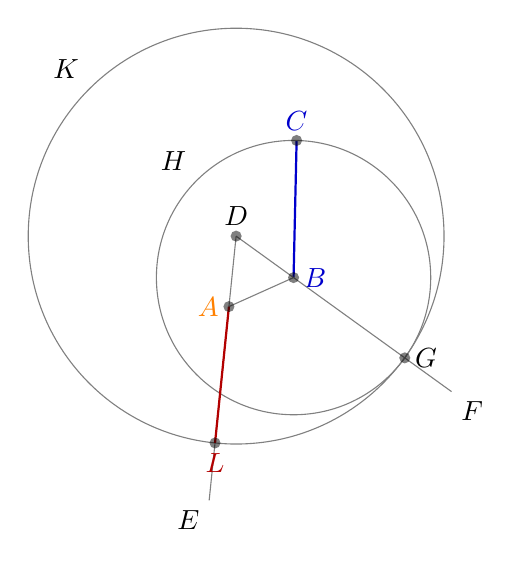
\begin{tikzpicture}[thick,help lines/.style={thin,draw=black!50}]
  \def\A{\textcolor{orange}{$A$}}   \def\B{\textcolor{input}{$B$}}
  \def\C{\textcolor{input}{$C$}}    \def\D{$D$}
  \def\E{$E$}                       \def\F{$F$}
  \def\G{$G$}                       \def\H{$H$}
  \def\K{$K$}                       \def\L{\textcolor{output}{$L$}}
  
  \colorlet{input}{blue!80!black}    \colorlet{output}{red!70!black}
  
  \coordinate [label=left:\A]  (A) at ($ (0,0) + .1*(rand,rand) $);
  \coordinate [label=right:\B] (B) at ($ (1,0.2) + .1*(rand,rand) $);
  \coordinate [label=above:\C] (C) at ($ (1,2) + .1*(rand,rand) $);

  \draw [input] (B) -- (C);
  \draw [help lines] (A) -- (B);

  \coordinate [label=above:\D] (D) at ($ (A)!.5!(B) ! {sin(60)*2} ! 90:(B) $);

  \draw [help lines] (D) -- ($ (D)!3.75!(A) $) coordinate [label=-135:\E] (E);
  \draw [help lines] (D) -- ($ (D)!3.75!(B) $) coordinate [label=-45:\F] (F);

  \node (H) at (B) [help lines,circle through=(C),draw,label=135:\H] {};

  \coordinate [label=right:\G] (G) at (intersection of B--F and H);

  \node (K) at (D) [help lines,circle through=(G),draw,label=135:\K] {};

  \coordinate [label=below:\L] (L) at (intersection of A--E and K);

  \draw [output] (A) -- (L);

  \foreach \point in {A,B,C,D,G,L}
    \fill [black,opacity=.5] (\point) circle (2pt);

  % \node ...
\end{tikzpicture}
\end{codeexample}